\chapter{暗物质、轴子与偏振量子通道}
\label{chap:e22}

\begin{chapteropening}
上一章（第 \ref{chap:e21} 章）我们把光一路飞来所受的传播改写全记了账：磁化等离子体让偏振面随 \(\lambda^2\) 拧转（法拉第旋转），引力透镜把像复制、移位、拉伸。请把那一章的结论记牢——那些等离子体前景和透镜通道，正是本章要找的新物理必须先甄别、再撬开的\emph{对照组}。而更早在第 \ref{chap:e18} 章我们还在磁星表面看到一件奇事：磁场强到接近临界场时，\emph{真空本身}都变成了一种有偏振方向的介质。那时留下一句话——偏振（polarization）是一条独立的量子通道，值得单独打开。这一章就来兑现它。新物理很少送给我们一张干净的"新粒子照片"；它更喜欢藏在偏振角的一次微小拧转里、藏在偏振随时间的缓慢摆动里、藏在强磁场里某个能段异常增亮的光子里。这一章的主角是轴子（axion）和轴子样粒子（axion-like particle，ALP）：它们通过一个极简单的耦合 \(a\,\bm E\cdot\bm B\) 与光对话，能让线偏振面转过一个角度，能让偏振信号随暗物质场一起振荡，还能在中子星、磁星和黑洞的强场环境里把一部分光"变"成或"变"走。我们的任务分三步：先把这个耦合翻译成一个能观测的旋转角，把它随耦合常数和传播路径的关系一步步写出来；再看看怎样用\emph{偏振分辨的强度与相干测量}去抓这个微弱到 \(10^{-3}\) 弧度甚至更小的信号；最后把它放回致密天体的强场里，问一句最要命的话——这到底是新物理，还是仪器和前景在骗我们？
\end{chapteropening}


\section{一个耦合，两个观测量：旋转与转换}
\label{sec:e22-coupling}

先把态度摆正：这一章不急着宣布"发现了轴子"。我们的做法始终是——先把"新物理"翻译成一个具体的观测量，再反过来问，普通天体物理和普通仪器能不能\emph{伪造}出同一个观测量。对轴子来说，最干净的两个入口都来自\emph{同一个}相互作用项：一个是线偏振面被轻轻拧转（旋转，rotation），另一个是在外磁场里轴子和光子互相变身（转换，conversion）。

在低能有效理论里，轴子样场 \(a\) 与电磁场的耦合写成

\begin{equation}
  \mathcal L_{a\gamma}
  = -\frac{1}{4}\,g_{a\gamma}\,a\,F_{\mu\nu}\tilde F^{\mu\nu}
  = g_{a\gamma}\,a\,\bm E\cdot\bm B .
  \label{eq:e22-lagrangian}
\end{equation}
\begin{formulaexplain}
\(a\)：轴子样场（能量量纲）；\(g_{a\gamma}\)：轴子--光子耦合常数，量纲 \(\mathrm{energy^{-1}}\)，天体文献惯用 \(\mathrm{GeV^{-1}}\)；\(F_{\mu\nu}\)、\(\tilde F^{\mu\nu}\)：电磁张量与它的对偶。写成 \(\bm E\cdot\bm B\) 后一眼看出：只有当电场、磁场取向"手性"相关时，这一项才起作用。
\end{formulaexplain}

把每个符号落到地上。\(F_{\mu\nu}\) 就是我们熟悉的电磁场张量，它的对偶 \(\tilde F^{\mu\nu}=\tfrac12\epsilon^{\mu\nu\alpha\beta}F_{\alpha\beta}\) 把电场和磁场对调了位置，所以 \(F\tilde F\propto \bm E\cdot\bm B\) 是一个赝标量（parity-odd）——它在空间反射下变号。轴子 \(a\) 也是赝标量，两者相乘才凑成一个真正的标量，才能进拉氏量。耦合常数 \(g_{a\gamma}\) 的大小是我们要测的靶心：天体和实验室的现有限制普遍把它压在 \(10^{-10}\text{--}10^{-12}\,\mathrm{GeV^{-1}}\) 这个量级以下。对严格的 QCD 轴子（QCD axion），质量与破缺尺度还锁在一条窄带上，

\begin{equation}
  m_a \simeq 5.7\,\mu\mathrm{eV}\left(\frac{10^{12}\,\mathrm{GeV}}{f_a}\right),
  \label{eq:e22-qcd-mass}
\end{equation}
\begin{formulaexplain}
\(m_a\)：轴子质量（能量单位，\(\mu\mathrm{eV}=10^{-6}\,\mathrm{eV}\)）；\(f_a\)：Peccei--Quinn 对称破缺尺度（GeV）。破缺尺度越高，轴子越轻。这条关系把 QCD 轴子钉在参数图上的一条斜带附近。
\end{formulaexplain}

其中 \(f_a\) 是 Peccei--Quinn 对称的破缺能标 \citep{1977PhRvL..38.1440P,1978PhRvL..40..223W,1978PhRvL..40..279W}。ALP 不必守这条规矩，\(m_a\) 和 \(g_{a\gamma}\) 可以近似独立，所以参数图上人们把"QCD 轴子带"和更宽的"ALP 参数空间"分开画 \citep{2016PhR...643....1M,2014JHEP...06..037D,1983PhRvL..51.1415S}。这一节先讲"旋转"，磁场里的"转换"留到第 \ref{sec:e22-strongfield} 节的强场环境里再算。


\section{把旋转角一步步算出来}
\label{sec:e22-rotation}

现在做本章最核心的一步推导：轴子背景到底怎样拧动线偏振面，拧过的角度和耦合常数、传播路径是什么关系。我们要把它算到不跳任何一步。

\paragraph{物理图像：左右手圆偏振跑得不一样快}

先给画面。一束线偏振光，可以想成两支反向旋转的圆偏振（circular polarization）叠加——一支左旋 \(\mathrm L\)、一支右旋 \(\mathrm R\)，两支旋转箭头的合成正好是一条来回摆动的直线，摆动的方向就是偏振面。关键在于：轴子耦合 \eqref{eq:e22-lagrangian} 是一个赝标量，它对左旋和右旋"不一视同仁"。左旋光走过一段路，相位比真空里\emph{多}积累一点；右旋光则\emph{少}积累一点。等两支箭头到达望远镜时，它们之间多出了一个相位差 \(\Delta\varphi\)。两支反向旋转、相位错开的箭头再合成，得到的还是一条直线——只不过这条直线整体转过了角度。这就是偏振旋转的全部秘密：\textbf{线偏振面的旋转，等于左右圆偏振相位差的一半}。

\paragraph{第一步：写出左右圆偏振的相位差}

轴子耦合让麦克斯韦方程多出一项源，从而改写光子的色散关系。这里我们\emph{直接引用}轴子--光子系统在几何光学（WKB）近似下的标准结果：对沿光线传播方向缓变的轴子背景 \(a(t,\bm x)\)，左右两个圆偏振模会各自获得一个正比于 \(\pm g_{a\gamma}\,\partial_\mu a\) 的波数移动（正负号按手性区分左右旋，这正是赝标量耦合"不一视同仁"的体现）。这条修正色散关系的完整推导属于场论范围，本书从略——读者只需知道它是被引用、而非应自行补出的一步。把这点波数偏移沿光线世界线积分，得到两支圆偏振累计的相位差

\begin{equation}
  \Delta\varphi \equiv \varphi_{\mathrm R}-\varphi_{\mathrm L}
  = g_{a\gamma}\!\int_{\rm src}^{\rm obs}\! \partial_\mu a\,\mathrm dx^\mu
  = g_{a\gamma}\,[\,a(t_o,\bm x_o)-a(t_e,\bm x_e)\,].
  \label{eq:e22-phase-diff}
\end{equation}
\begin{formulaexplain}
\(\Delta\varphi\)：右旋减左旋的累计相位差（无量纲）；积分沿光子从发射点（\(e\)）到观测点（\(o\)）的路径。因为被积的是全微分 \(\partial_\mu a\,\mathrm dx^\mu=\mathrm da\)，积分只留下两端点场值之差，路径中间怎么弯都被抵消。
\end{formulaexplain}

这一步最漂亮的地方，是那个积分号里装的是\emph{全微分}。沿光子世界线，\(\partial_\mu a\,\mathrm dx^\mu\) 就是 \(a\) 沿这条线的微小变化 \(\mathrm da\)；一路加起来，只剩起点和终点的差 \(a_o-a_e\)。这带来一个立刻能用的结论：\textbf{旋转只认发射端和接收端的轴子场值，不认中间走了多长}。中间即使穿过一片来回起伏的轴子场，起伏也在积分里自相抵消。这和下一节磁场里的"转换"截然相反——转换是沿程累积的，走得越长（相干范围内）信号越强。请把这两种"距离依赖"记牢，它们后面是区分信号来源的利器。

\paragraph{第二步：相位差的一半就是旋转角}

现在把 \(\Delta\varphi\) 翻译成偏振面的旋转角。把一束沿 \(x\) 方向的线偏振光写成左右圆偏振的等幅叠加，\(\hat{\bm e}_{\mathrm R}=(\hat{\bm x}-i\hat{\bm y})/\sqrt2\)、\(\hat{\bm e}_{\mathrm L}=(\hat{\bm x}+i\hat{\bm y})/\sqrt2\)，于是

\[
  \bm E \propto \hat{\bm e}_{\mathrm R}\,e^{i\varphi_{\mathrm R}}
              +\hat{\bm e}_{\mathrm L}\,e^{i\varphi_{\mathrm L}}
  = e^{i\bar\varphi}\Big[\hat{\bm e}_{\mathrm R}\,e^{+i\Delta\varphi/2}
                        +\hat{\bm e}_{\mathrm L}\,e^{-i\Delta\varphi/2}\Big],
\]

其中 \(\bar\varphi=(\varphi_{\mathrm R}+\varphi_{\mathrm L})/2\) 是公共相位、可以提出来丢掉。把方括号里的圆偏振基代回直角基，用 \(\hat{\bm e}_{\mathrm R}e^{i\theta}+\hat{\bm e}_{\mathrm L}e^{-i\theta}=\sqrt2\,(\hat{\bm x}\cos\theta+\hat{\bm y}\sin\theta)\)（\(\theta=\Delta\varphi/2\)），方括号正好是一条指向 \((\cos\theta,\sin\theta)\) 的直线。也就是说偏振面从 \(x\) 轴转过了 \(\theta=\Delta\varphi/2\)。于是

\begin{equation}
  \Delta\psi = \frac{\Delta\varphi}{2}
  = \frac{1}{2}\,g_{a\gamma}\,[\,a(t_o,\bm x_o)-a(t_e,\bm x_e)\,].
  \label{eq:e22-rotation}
\end{equation}
\begin{formulaexplain}
\(\Delta\psi\)：线偏振面的旋转角（弧度）。它等于左右圆偏振相位差的一半，正比于耦合 \(g_{a\gamma}\) 与两端轴子场之差。注意式中\emph{没有}波长——这是它和法拉第旋转最要命的区别。
\end{formulaexplain}

逐项落地。\(\Delta\psi\) 是弧度；\(g_{a\gamma}\)（\(\mathrm{GeV^{-1}}\)）越大、两端场值差越大，旋转越明显。最值得反复念的一点是：\eqref{eq:e22-rotation} 里\textbf{不含波长 \(\lambda\)}，所以轴子旋转是\emph{无色的}（achromatic）。请回忆第 \ref{chap:e21} 章的法拉第旋转（Faraday rotation）\(\psi=\psi_0+\mathrm{RM}\,\lambda^2\)，它随 \(\lambda^2\) 变。这一条波长依赖的差别，就是我们在真实数据里把轴子信号和等离子体前景撬开的\emph{第一把撬棍}：测几个频率，看旋转角随不随 \(\lambda^2\) 走。若随，多半是法拉第；若几乎不随频率变、却随\emph{时间}摆动，才轮到轴子上场。


\section{振荡的偏振：暗物质是一支缓慢转动的指针}
\label{sec:e22-oscillation}

\eqref{eq:e22-rotation} 只说旋转正比于场值之差，还没说这个场随时间怎么动。如果轴子恰好就是本地的超轻暗物质（ultralight dark matter），那么这个"场值之差"会随时间振荡，把一个静止的旋转角变成一条会呼吸的时间序列——这正是偏振作为量子通道最独特的签名。

一团冷的超轻暗物质，在本地近似是一个相干振荡的经典场：

\begin{equation}
  a(t,\bm x)\simeq a_0\cos(m_a t+\varphi),
  \qquad
  a_0=\frac{\sqrt{2\rho_a}}{m_a}.
  \label{eq:e22-dm-field}
\end{equation}
\begin{formulaexplain}
\(a_0\)：场振幅；\(\rho_a\)：本地暗物质能量密度（银河系取 \(0.3\,\mathrm{GeV\,cm^{-3}}\) 作量级）；\(m_a\)：轴子质量。质量越小，同样能量密度下场振幅越大——轻轴子的偏振摆动更大、也更慢。
\end{formulaexplain}

这条式子的物理是能量密度守恒：一个质量 \(m_a\) 的场，能量密度约 \(\rho_a\sim\tfrac12 m_a^2 a_0^2\)，反解就得 \(a_0=\sqrt{2\rho_a}/m_a\)。质量越轻，要凑够同样的 \(\rho_a\)，场振幅 \(a_0\) 就得越大——所以\emph{越轻的轴子，偏振旋转的幅度越大}。把 \eqref{eq:e22-dm-field} 代进旋转公式 \eqref{eq:e22-rotation}，观测端的旋转角就随时间振荡：

\begin{equation}
  \Delta\psi(t)\simeq \tfrac12\,g_{a\gamma}\,a_0
  \big[\cos(m_a t_o+\varphi)-\cos(m_a t_e+\varphi)\big],
  \label{eq:e22-osc-signal}
\end{equation}
\begin{formulaexplain}
观测端旋转角随时间做正弦摆动，幅度约 \(\tfrac12 g_{a\gamma}a_0\)，角频率就是轴子质量 \(m_a\)（自然单位下 \(\omega=m_ac^2/\hbar\)）。发射端那一项在远源时以推迟时间振荡，通常与观测端不同步。
\end{formulaexplain}

它的振荡周期和相干时间是

\begin{equation}
  T_a=\frac{2\pi\hbar}{m_ac^2}\simeq 47.9\,\mathrm{d}\left(\frac{10^{-21}\,\mathrm{eV}}{m_a}\right),
  \qquad
  t_{\rm coh}\sim\frac{T_a}{v^2},
  \label{eq:e22-timescales}
\end{equation}
\begin{formulaexplain}
\(T_a\)：偏振摆动周期；\(t_{\rm coh}\)：场保持同一相位的相干时间；\(v\sim10^{-3}c\)：银河晕的速度弥散。超轻质量对应很长的周期，而弥散很小，所以同一频率的相位能撑过许多个周期。
\end{formulaexplain}

代个真实数字体会一下。取 \(m_a=10^{-21}\,\mathrm{eV}\)，偏振面会以约 \(48\) 天的周期来回拧动；因为暗物质速度弥散只有 \(v\sim10^{-3}c\)，相干时间 \(t_{\rm coh}\sim T_a/v^2\) 长到 \(10^5\) 年量级——也就是说，在人类的整个观测史里，这个"频率"稳如一台超稳时钟，相位几乎不漂。这把搜寻策略指得很明确：不要只测一次偏振角，要在\emph{几十天到几年}的时间基线上反复测同一批源，找那条共同的、准单频的正弦摆动。这也解释了为什么"静态的宇宙双折射搜索"并不等价于"振荡的暗物质搜索"：前者找一个不随时间变的常数角，后者找一条会呼吸的曲线。Fedderke、Graham 与 Rajendran 正是据此指出，超轻轴子暗物质会在最后散射面留下 washout、在今天的偏振里留下共同振荡，两者是不同的观测通道 \citep{2019PhRvD.100a5040F,2021ARA&A..59..247H}。

\begin{figure}[tbp]
\centering
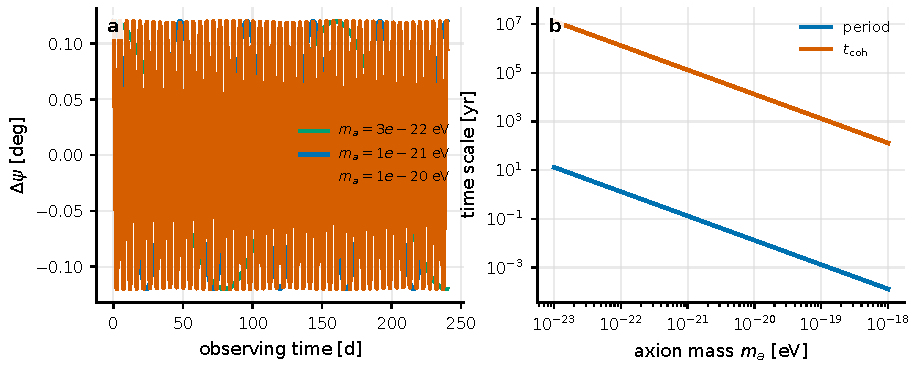
\includegraphics[width=0.94\linewidth]{figures/generated/chapter_15/ch15_axion_polarization_oscillation.pdf}
\caption{超轻暗物质把偏振旋转变成时间序列。左图画出三个轴子质量对应的 \(\Delta\psi(t)\)：质量越大、振荡越快。右图把质量 \(m_a\) 换算成周期 \(T_a\) 和相干时间 \(t_{\rm coh}\sim T_a/v^2\)（取 \(v=10^{-3}c\)）：越轻的轴子摆得越慢，却能在越长的时间里保持同一相位。}
\label{fig:e22-oscillation}
\end{figure}


\section{怎样测这么小的旋转：偏振分辨的强度与相干测量}
\label{sec:e22-measure}

目标信号常常小到 \(10^{-3}\) 弧度甚至更小。这一节要说清楚：我们凭什么、用什么数据结构去抓它，以及为什么"抓到一个非零角"往往首先是一个\emph{系统误差}问题，而不是发现。

\paragraph{偏振测量的本质：在偏振基上数光子}

回到第 \ref{chap:e18} 章打下的地基：偏振测量的本质，就是把一束光分到两个（或几个）正交偏振通道里，\emph{分别数光子}。用斯托克斯参量（Stokes parameters）\(I,Q,U,V\) 记账，线偏振信息全在 \(Q\)、\(U\) 里。一次偏振旋转 \(\beta\) 对 \(Q,U\) 的作用极其干净：把复组合 \(Q\pm iU\) 乘上一个相位因子，

\begin{equation}
  Q\pm iU \;\longrightarrow\; e^{\pm 2i\beta}\,(Q\pm iU).
  \label{eq:e22-qu-rotation}
\end{equation}
\begin{formulaexplain}
\(Q,U\)：线偏振斯托克斯参量；\(\beta\)：整体偏振旋转角。指数里那个 \(2\beta\)（不是 \(\beta\)）来自线偏振的"自旋 2"性质——偏振是一条无向的双箭头，转 \(180^\circ\) 就复原，所以数学上以 \(2\beta\) 出现。
\end{formulaexplain}

那个 \(2\) 很关键：它意味着一个很小的角度误差就足以让本该干净的模式互相污染。在球谐（\(E/B\) 模）空间里，\eqref{eq:e22-qu-rotation} 会把 \(E\) 模漏进 \(B\) 模。若源本身的奇宇称谱可忽略，旋转后出现的奇宇称谱近似为

\begin{equation}
  C_\ell^{EB,\rm obs}=\tfrac12\sin(4\beta)\,(C_\ell^{EE}-C_\ell^{BB}),
  \qquad
  C_\ell^{TB,\rm obs}=\sin(2\beta)\,C_\ell^{TE}.
  \label{eq:e22-eb-tb}
\end{equation}
\begin{formulaexplain}
\(C_\ell^{EB},C_\ell^{TB}\)：旋转后冒出来的奇宇称功率谱；\(\beta\)：旋转角。若源本征的 \(EB/TB\) 很小，非零的 \(EB/TB\) 就成了旋转角的探针——但探测器角度标定的错误会产生几乎一模一样的形状。
\end{formulaexplain}

\paragraph{宇宙双折射：为什么它首先是角标定问题}

宇宙微波背景（CMB）是找"全局偏振旋转"的诱人靶子：最后散射面极远，天区极大，统计量能压到很小。可它也把一个简单问题逼成最尖锐的系统误差问题。宇宙本身把偏振转了 \(\beta\)（宇宙双折射，cosmic birefringence），和探测器整体角度标定错了 \(\alpha\)，在 CMB 谱里长得几乎一样——两者都通过 \eqref{eq:e22-eb-tb} 冒出同样形状的 \(EB\)。代个数感受强度：\(\beta=0.35^\circ\) 时 \(\tfrac12\sin(4\beta)\simeq0.012\)，也就是 \(EB\) 泄漏只有 \(EE\!-\!BB\) 的百分之一量级——信号本就微弱，还和标定误差纠缠在一起。Planck 2018 的重新分析靠一个巧办法把两者部分撬开：CMB 旋转 \(\beta\) 只作用于最后散射面来的光，而银河前景偏振近在眼前、\emph{不}被宇宙旋转拧过，两者对频率和多极矩的依赖不同，于是可以同时拟合 \(\beta\) 和标定角 \(\alpha\)，给出 \(\beta=0.35\pm0.14^\circ\)（\(68\%\) 置信）。后续 WMAP+Planck、Planck PR4 的分析反复强调，尘埃自身的 \(EB\)、带通失配、\(I\to P\) 泄漏、交叉偏振响应和天区掩模的选择，仍是压在这个结果上的主要系统误差 \citep{2020PhRvL.125v1301M,2022NatRP...4..452K,2022PhRvD.106f3503E,2022PhRvL.128i1302D}。宇宙双折射的原始理论根据，可追到 Carroll、Field、Jackiw 等对赝标量场诱导旋光的讨论 \citep{1990PhRvD..41.1231C,1999PhRvL..83.1506L}。

\begin{figure}[tbp]
\centering
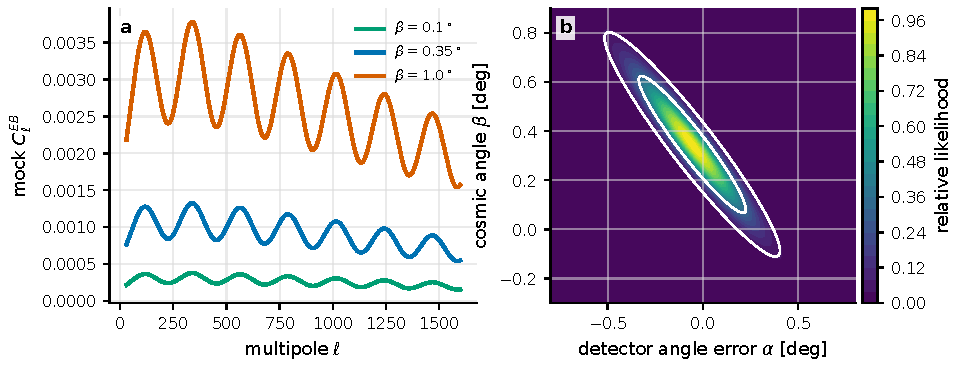
\includegraphics[width=0.94\linewidth]{figures/generated/chapter_15/ch15_cosmic_birefringence.pdf}
\caption{宇宙双折射同时牵动 \(E/B\) 混合与仪器角标定。左图用玩具 \(EE\)、\(BB\) 谱演示旋转角 \(\beta\) 怎样凭空生出 \(EB\)。右图画出标定角 \(\alpha\) 与宇宙旋转 \(\beta\) 的退化：只看 CMB，两者几乎等价；靠前景的频率依赖，才能把退化部分打破。}
\label{fig:e22-birefringence}
\end{figure}

\paragraph{把测量保留成事件表：不要过早平均}

\Needspace{10\baselineskip}
更一般地，最稳妥的做法是别急着把数据平均成"一张固定偏振角的图"，而是保留成一份\emph{偏振事件表}（沿用第 \ref{chap:e13} 章的事件表范式）。每个光子事件带上时间、频率、方向、偏振通道和权重：

\begin{equation}
  e_q=(t_q,\ \nu_q,\ \hat{\bm n}_q,\ p_q,\ w_q).
  \label{eq:e22-event}
\end{equation}
\begin{formulaexplain}
\(e_q\)：第 \(q\) 个偏振事件；\(t_q,\nu_q,\hat{\bm n}_q\)：到达时间、频率、天球方向；\(p_q\)：落进哪个偏振通道；\(w_q\)：质量权重。保留成事件表，就能在时间和频率维度上同时找"共同旋转"，而不必先把相位信息平均掉。
\end{formulaexplain}

若偏振角里藏着一个小的公共振荡 \(\delta\psi\)，落进某个偏振通道的概率就写成

\begin{equation}
  P\!\left(p_q\,\middle|\,t_q,\nu_q,\hat{\bm n}_q\right)
  = P_0\!\left[\,p_q\,\middle|\,\psi_{\rm src}
     +\psi_{\rm prop}(\nu_q,\hat{\bm n}_q)+\delta\psi(t_q,\hat{\bm n}_q)\,\right].
  \label{eq:e22-likelihood}
\end{equation}
\begin{formulaexplain}
\(\psi_{\rm src}\)：源本征偏振角；\(\psi_{\rm prop}\)：传播与仪器项（含法拉第、尘埃、仪器 Mueller 矩阵）；\(\delta\psi\)：要检验的新物理旋转。这条似然把"异常角度"拆成几类\emph{可以互相反驳}的来源，一起放进同一个拟合。
\end{formulaexplain}

代价也直白得吓人：如果仪器的 Mueller 矩阵非对角项只标定到 \(10^{-3}\)，而你要找的旋转也是 \(10^{-3}\) 弧度，那么系统误差已经和信号\emph{同量级}——这时候一个漂亮的非零角，多半是仪器在说话，不是宇宙。孤立中子星的光学偏振、磁星的 X 射线偏振、以及强场 QED 真空双折射的候选信号，都必须先把源的几何和传播效应建模干净，偏振异常才可能被解释成新物理 \citep{2017MNRAS.465..492M}。


\section{强场环境：致密天体作为轴子实验室}
\label{sec:e22-strongfield}

旋转通道靠的是轴子场本身；\emph{转换}通道则要借一片强磁场，把轴子和光子直接互相变身。哪里有最强的磁场？正是第 \ref{chap:e18} 章的致密天体（中子星、磁星）与第 \ref{chap:e19} 章的黑洞。这一节把偏振量子通道搬进中子星、磁星和黑洞的强场环境，既算转换概率，也接上超辐射的玻色云。

\paragraph{磁场里的轴子--光子转换}

在横向磁场 \(B_\perp\) 中，轴子只和与 \(B_\perp\) 平行的那个光子偏振态混合。弱混合、均匀磁场、吸收可忽略时，转换概率是

\begin{equation}
  P_{a\to\gamma}\simeq\left(\frac{g_{a\gamma}B_\perp L}{2}\right)^2
  \mathrm{sinc}^2\!\left(\frac{qL}{2}\right),
  \qquad
  q\simeq\frac{|m_a^2-m_\gamma^2|}{2E}.
  \label{eq:e22-conversion}
\end{equation}
\begin{formulaexplain}
\(P_{a\to\gamma}\)：轴子变光子的概率；\(B_\perp\)：横向磁场；\(L\)：相干路径长；\(E\)：能量；\(m_\gamma\)：等离子体里光子的有效质量；\(q\)：轴子与光子的动量失配。前面的平方给强度，\(\mathrm{sinc}^2\) 因子管相干：相位一失配，累积就被砍断。
\end{formulaexplain}

请把它和旋转公式 \eqref{eq:e22-rotation} 并排看，两种"距离依赖"的对比一目了然。当 \(qL\ll1\)（相干），\(\mathrm{sinc}^2\to1\)，概率按 \(L^2\) 增长——\textbf{转换是沿程累积的，走得越长越强}，这正好和"旋转只认两端点"相反。可一旦 \(qL\gtrsim\pi\)，不同路径段的转换振幅开始反相抵消，\(\mathrm{sinc}^2\) 迅速衰减，再长也没用。这就是相干长度的物理。地面实验把这个公式用到极致：CAST 用一块退役的 LHC 偶极磁体（\(9\,\mathrm T\)、\(9.26\,\mathrm m\)）盯着太阳，找太阳轴子转换成的 X 射线，其 2013--2015 真空管数据给出 \(g_{a\gamma}<0.66\times10^{-10}\,\mathrm{GeV^{-1}}\)（\(95\%\) 置信），适用于 \(m_a\lesssim0.02\,\mathrm{eV}\) 的相干低质量区 \citep{2017NatPh..13..584C}。

\begin{figure}[tbp]
\centering
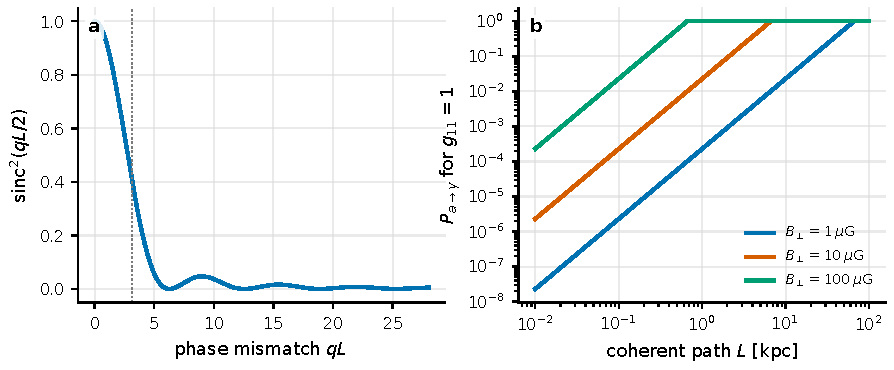
\includegraphics[width=0.94\linewidth]{figures/generated/chapter_15/ch15_axion_conversion.pdf}
\caption{轴子--光子转换由强度和相位共同决定。左图是相干因子 \(\mathrm{sinc}^2(qL/2)\)：当 \(qL\) 逼近 \(\pi\)，路径不同部分的转换振幅开始抵消。右图给出星际尺度的相干极限量级（取 \(g_{a\gamma}=10^{-11}\,\mathrm{GeV^{-1}}\)）：在 \(\mu\mathrm G\) 磁场、kpc 路径下，单段转换概率通常远小于 1。}
\label{fig:e22-conversion}
\end{figure}

\paragraph{磁星与 FRB：极端磁化的偏振实验室}

中子星和磁星把这一切推到极限——第 \ref{chap:e18} 章我们已经看到，磁星表面的磁场逼近临界场，连真空都成了双折射介质。这种环境对轴子转换是天然的放大器，但也意味着本征的偏振结构和传播前景都极强。快速射电暴（FRB）给了另一类极端样本：FRB~121102 落在 \(z=0.193\) 的宿主星系里，\(4\text{--}8\,\mathrm{GHz}\) 的暴发显示近乎 \(100\%\) 的线偏振，却带着高得离谱、还随时间变的法拉第旋转量 \(\mathrm{RM}_{\rm src}=1.46\times10^5\) 与 \(1.33\times10^5\,\mathrm{rad\,m^{-2}}\)，个别子结构窄到 \(\lesssim30\,\mu\mathrm s\)。若宿主贡献 \(\mathrm{DM_{host}}\sim70\text{--}270\,\mathrm{pc\,cm^{-3}}\)，反推出的视线磁场下限已达毫高斯（mG）量级，是普通银河系星际介质 \(\sim5\,\mu\mathrm G\) 的几百倍 \citep{2018Natur.553..182M}。这类源既是极端磁化等离子体的实验室，也是最狡猾的骗子：一个看似"无色"的偏振变化，仍要先排除有限通道宽度造成的退偏振、\(\mathrm{RM}\) 随时间漂移、以及等离子体透镜的选择效应，才轮到轴子。

\begin{figure}[tbp]
\centering
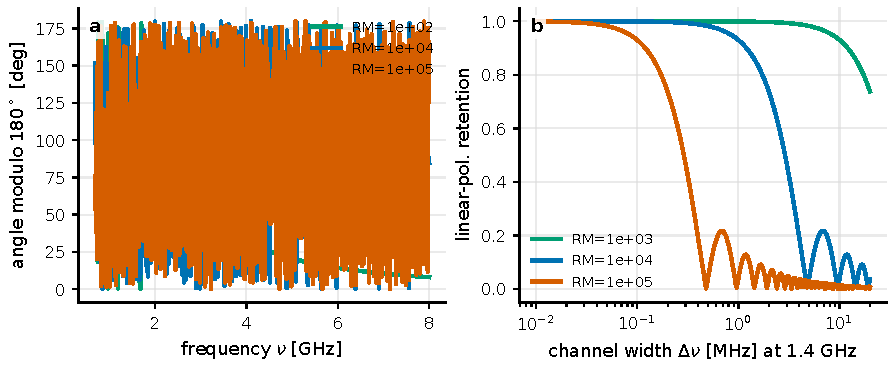
\includegraphics[width=0.94\linewidth]{figures/generated/chapter_15/ch15_frb_faraday_foreground.pdf}
\caption{FRB 的偏振前景能轻松淹没微弱旋转。左图画出不同 \(\mathrm{RM}\) 下偏振角随频率的 \(180^\circ\) 缠绕：\(\mathrm{RM}=10^5\,\mathrm{rad\,m^{-2}}\) 在 GHz 频段变化极快。右图是 \(1.4\,\mathrm{GHz}\) 附近有限通道宽度造成的线偏振保留率——要测这么高的 \(\mathrm{RM}\)，必须用极窄的通道。}
\label{fig:e22-frb}
\end{figure}

\paragraph{黑洞超辐射：把轻玻色场种在自转黑洞旁}

黑洞把轻玻色场和偏振图像连成一体。绕着自转（Kerr）黑洞的玻色波，只要频率足够低，满足

\begin{equation}
  \omega<m\,\Omega_H,
  \label{eq:e22-superradiance}
\end{equation}
\begin{formulaexplain}
\(\omega\)：玻色模频率；\(m\)：方位量子数（整数）；\(\Omega_H\)：Kerr 黑洞视界的角速度。满足这条不等式时，波会从黑洞自转里\emph{抽}走能量，指数增长，堆成一团绕黑洞旋转的玻色云。
\end{formulaexplain}

就能从黑洞自转里抽能量，指数放大，长成一团"超辐射玻色云"（superradiant boson cloud）。云能不能有效长起来，取决于轴子康普顿波长与黑洞尺度是否匹配。定义一个无量纲的"引力精细结构常数"

\begin{equation}
  \alpha_G=\frac{G M_\bullet m_a}{\hbar c},
  \label{eq:e22-alphaG}
\end{equation}
\begin{formulaexplain}
\(\alpha_G\)：黑洞引力半径与轴子康普顿波长之比；\(M_\bullet\)：黑洞质量。当 \(\alpha_G\sim0.1\text{--}1\) 时，玻色波"装得进"黑洞附近，超辐射增长最快。
\end{formulaexplain}

当 \(\alpha_G\sim0.1\text{--}1\)，玻色康普顿波长与黑洞尺度对上，云长得最凶。把 \eqref{eq:e22-alphaG} 反解，就把黑洞质量映射到它最敏感的轴子质量：

\begin{equation}
  m_a\simeq 1.34\times10^{-10}\,\mathrm{eV}\;\alpha_G
  \left(\frac{M_\odot}{M_\bullet}\right).
  \label{eq:e22-bh-mass}
\end{equation}
\begin{formulaexplain}
把黑洞质量 \(M_\bullet\) 换算成最敏感的轴子质量 \(m_a\)：黑洞越重，对应的轴子质量窗口越低。所以不同质量的黑洞，探的是超轻质量谱的不同段。
\end{formulaexplain}

代两个真实黑洞。银心 Sgr~A\(^*\)（\(4.3\times10^6\,M_\odot\)）在 \(\alpha_G=0.4\) 时对应 \(m_a\simeq1.2\times10^{-17}\,\mathrm{eV}\)；M87\(^*\)（\(6.5\times10^9\,M_\odot\)）则对应 \(8\times10^{-21}\,\mathrm{eV}\)——两个黑洞探的是完全不同的质量段。这里偏振通道又回来了：EHT 的偏振成像里，轴子云会让环上的偏振角随轴子周期一起摆动，Sgr~A\(^*\) 的周期约 \(100\text{--}1000\,\mathrm s\)，M87\(^*\) 可长到数天。能不能看见这种摆动，取决于空间分辨率——若分辨不开环上不同方位，摆动就会被"平均"抹平 \citep{2015LNP...906.....B,2015CQGra..32m4001B,2017PhRvD..96c5019B,2020PhRvL.124f1102C,2022NatAs...6..592C}。

\begin{figure}[tbp]
\centering
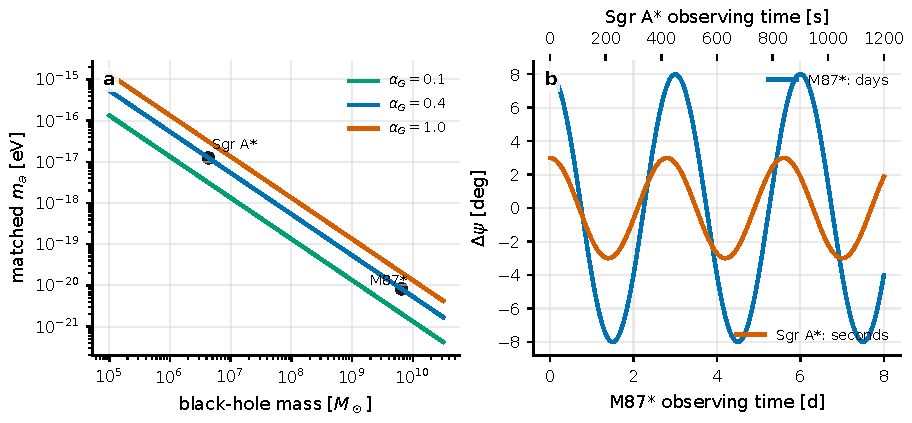
\includegraphics[width=0.94\linewidth]{figures/generated/chapter_15/ch15_black_hole_axion_cloud.pdf}
\caption{黑洞质量框定超辐射轴子的质量窗口。左图用 \(\alpha_G=GM_\bullet m_a/\hbar c\) 标出不同黑洞质量对应的 \(m_a\)：Sgr~A\(^*\) 与 M87\(^*\) 落在不同的超轻质量段。右图给出 EHT 偏振角振荡的两个典型时标：M87\(^*\) 可在天尺度采样，Sgr~A\(^*\) 则需要秒到分钟级的偏振成像。}
\label{fig:e22-bh}
\end{figure}


\section{把异常写成可反驳的检验}
\label{sec:e22-falsifiable}

走到这里，所有候选信号都共享一条铁律：\textbf{异常本身不是结论，异常的"可反驳结构"才是结论}。这一节把前面散落的招数收成一套统一的账本。

\paragraph{一份账本：把四类来源摊开对齐}

新物理搜索的观测量往往不止一个：偏振角、到达时间、像位置、放大率，可能来自不同仪器，各带各的统计与系统误差。把它们并成一个数据向量 \(\bm d\)，模型就拆成四大块：

\begin{equation}
  \bm m(\bm\theta)=\bm m_{\rm src}+\bm m_{\rm prop}+\bm m_{\rm inst}+\bm m_{\rm new}(\bm\theta),
  \label{eq:e22-model-vector}
\end{equation}
\begin{formulaexplain}
\(\bm m\)：模型预测向量；四项分别是源、传播、仪器、新物理。\(\bm\theta\)：新物理参数（\(g_{a\gamma}\)、\(m_a\)、\(\beta\)、子晕质量函数等）。这种拆分逼着我们把异常和普通天体物理、传播前景、校准误差摆进\emph{同一本账}里比较。
\end{formulaexplain}

在高斯近似下，拟合的目标函数是

\begin{equation}
  -2\ln\mathcal L=\big[\bm d-\bm m(\bm\theta)\big]^{\mathsf T}
  \big(C_{\rm stat}+C_{\rm sys}\big)^{-1}
  \big[\bm d-\bm m(\bm\theta)\big]
  +\ln\det\big(C_{\rm stat}+C_{\rm sys}\big).
  \label{eq:e22-likelihood-gauss}
\end{equation}
\begin{formulaexplain}
\(\mathcal L\)：高斯似然；\(C_{\rm stat}\)：统计协方差（光子噪声、到达时间误差、图像噪声）；\(C_{\rm sys}\)：系统误差协方差（Mueller 矩阵、绝对偏振角、法拉第前景、尘埃 \(EB\)、透镜宏模型……）。残差必须用两类误差\emph{一起}加权；漏掉 \(C_{\rm sys}\)，一个孤立异常就会被错误放大。
\end{formulaexplain}

这条式子把本章反复念叨的那句话数学化了：只要 \(C_{\rm sys}\) 没进似然，任何单个异常点都会被过度解释。

\paragraph{五把撬棍：让不同信号互相出卖}

好在这些信号有清清楚楚的相互区分方式，每一把都对应前面讲过的物理：

\begin{itemize}
\item \textbf{波长依赖。} 法拉第旋转随 \(\lambda^2\)（第 \ref{chap:e21} 章），轴子旋转近似无色（\eqref{eq:e22-rotation}）——测几个频率就能撬开。
\item \textbf{时间行为。} 静态宇宙双折射给一个不变的全局角（\eqref{eq:e22-eb-tb}），超轻暗物质给一条会呼吸的正弦（\eqref{eq:e22-osc-signal}）——测几十天到几年就能撬开。
\item \textbf{黑洞标度。} 超辐射云的偏振振荡应随黑洞质量、自转、环上方位和观测时间联动（\eqref{eq:e22-bh-mass}），普通吸积流不会这么"听黑洞的话"。
\item \textbf{路径依赖。} 转换按 \(L^2\) 沿程累积（\eqref{eq:e22-conversion}），旋转只认两端点——两者的距离响应正好相反。
\item \textbf{交叉检验。} 样本统计、空场或控制源、频率反演、时间相干性、仪器重标定，任何一项翻车，"发现"就该降级。
\end{itemize}

\paragraph{一个平行的通道：暗物质如何把质量变成角偏移}

偏振通道找的是"场对光子的量子影响"；还有一条平行的通道，找的是"暗物质质量分布对光线路径的影响"——引力透镜。它同样"无色"，同样不表现为"看到一团暗物质"，而表现为像位置、放大率或到达时间偏离普通模型。暗物质的存在本身有星系团碰撞（如子弹星团中弱透镜质量峰与 X 射线气体的分离，说明主质量近似无碰撞）、弱透镜和动力学多重支撑 \citep{2006ApJ...648L.109C,1993ApJ...404..441K}；而冷暗物质模拟预言银河晕里布满远低于可见卫星星系的子晕，成了强透镜异常的重要候选解释 \citep{1994ApJ...427L...1F,1999ApJ...524L..19M,2008Natur.454..735D}。子晕透镜的量级由爱因斯坦角给出，

\begin{equation}
  \theta_E=\left(\frac{4GM}{c^2}\frac{D_{ls}}{D_lD_s}\right)^{1/2},
  \qquad
  \delta\theta\simeq\frac{\theta_E^2}{b},
  \label{eq:e22-lensing}
\end{equation}
\begin{formulaexplain}
\(\theta_E\)：子晕爱因斯坦角，\(\propto M^{1/2}\)；\(M\)：透镜质量；\(D\)：观测者--透镜--源的距离组合；\(\delta\theta\)：像的天体测量偏移；\(b\)：像到子晕的角距离（\(b\gg\theta_E\)）。质量越大、越靠近像，位置扰动越明显；远离时按 \(1/b\) 衰减。
\end{formulaexplain}

数字把分辨率要求摆得很硬：在 \(D_l\simeq1\,\mathrm{Gpc}\)、\(D_s\simeq2\,\mathrm{Gpc}\) 的星系强透镜里，\(10^8\,M_\odot\) 子晕的 \(\theta_E\) 是几十毫角秒（mas），\(10^6\,M_\odot\) 只有几 mas；而 \(10^6\,M_\odot\) 子晕在 \(b=10\,\mathrm{mas}\) 处给出的天体测量偏移仅 \(\mu\mathrm{as}\) 量级。强透镜的流量比异常对放大率扰动敏感——Mao 与 Schneider 指出低质量子结构能解释一些四像系统的异常，Dalal 与 Kochanek 用 7 个射电透镜测得子结构质量分数中位数 \(f_{\rm sat}\simeq0.02\)（\(90\%\) 范围约 \(0.006\text{--}0.07\)），Vegetti、Hezaveh 等更用引力成像和 ALMA 把单个暗子结构的探测推进到空间分辨建模 \citep{1998MNRAS.295..587M,2002ApJ...572...25D,2010MNRAS.408.1969V,2016ApJ...823...37H}；Gaia 及未来天体测量巡天则把子晕横穿背景源变成时间域信号，主要限制来自扫描定律、源密度与自行协方差 \citep{2024MNRAS.531..632M,2016PhRvD..94h3504C}。这条通道与偏振通道的账本完全一致（\eqref{eq:e22-model-vector}）：暗子晕应\emph{同时}扰动像位置、放大率和时间延迟，而恒星表面结构主要随源自转、波长和基线方向变化——把这些区别放进同一个似然，异常才可能升格为发现。

\begin{figure}[tbp]
\centering
\includegraphics[width=0.94\linewidth]{figures/generated/chapter_15/ch15_dark_matter_lensing.pdf}
\caption{暗物质子晕的透镜信号受角尺度限制。左图给出典型 Gpc 几何下子晕爱因斯坦角随质量的变化。右图把 \(\delta\theta\simeq\theta_E^2/b\) 换成天体测量偏移：低质量子晕需要 mas 级的接近和 \(\mu\mathrm{as}\) 级的系统控制才可能看见。}
\label{fig:e22-lensing}
\end{figure}

\paragraph{一条时间域的旁证：脉冲星阵列}

同样的"共同时间项"逻辑，还能用在脉冲星身上。脉冲星有稳定相位、重复脉冲，天然适合做时间域阵列（脉冲星计时阵列，PTA）。超轻标量暗物质的引力势振荡会在计时残差里留下窄带信号：写成 \(\Psi_c\cos(2m_at+\varphi)\)，简化残差是

\begin{equation}
  R_\alpha(t)\simeq\frac{\Psi_c}{2\pi f}
  \Big[\sin(2\pi ft+\varphi_E)-\sin\!\big(2\pi f(t-D_\alpha/c)+\varphi_\alpha\big)\Big],
  \label{eq:e22-pta}
\end{equation}
\begin{formulaexplain}
\(R_\alpha\)：第 \(\alpha\) 颗脉冲星的计时残差；\(\Psi_c\)：势振荡幅度；\(f\simeq m_a/\pi\)：窄带频率；\(D_\alpha\)：脉冲星距离。第一项是所有脉冲星共享的"地球项"，第二项是每颗星各自的"脉冲星项"。
\end{formulaexplain}

\(m_a\sim10^{-23}\,\mathrm{eV}\) 对应 \(f\sim10^{-8}\,\mathrm{Hz}\)，正落在 PTA 的 \(10^{-9}\text{--}10^{-7}\,\mathrm{Hz}\) 窗口里。Porayko 与 Postnov 分析 NANOGrav 旧数据，给出 \(\Psi_c<1.14\times10^{-15}\)（\(95\%\) 置信）的上限 \citep{2014PhRvD..90f2008P}。这个标量模板的脉冲星间相关几乎不依赖两星夹角，因此不同于随机引力波背景那条著名的 Hellings--Downs 角相关曲线——这本身又是一把撬棍。若将来做"脉冲星偏振阵列"，同样要把共同地球项、本征磁层偏振、星际法拉第旋转、脉冲轮廓变化和接收机偏振泄漏一一分开。

\begin{figure}[tbp]
\centering
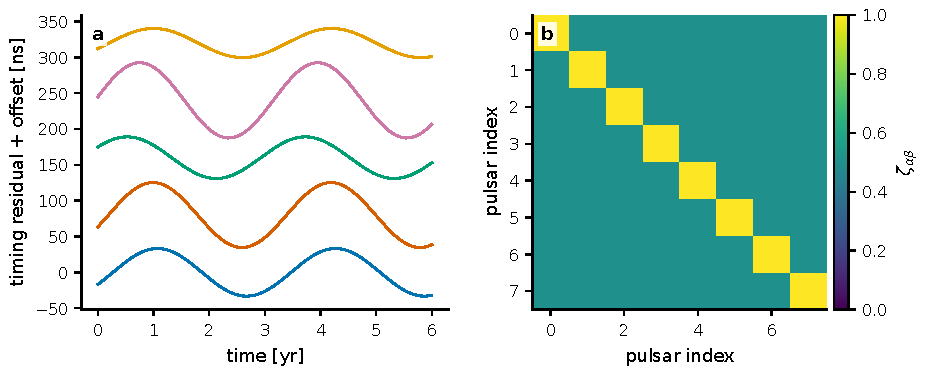
\includegraphics[width=0.94\linewidth]{figures/generated/chapter_15/ch15_pulsar_array_correlation.pdf}
\caption{脉冲星阵列里的共同窄带信号。左图是一个公共地球项叠加每颗星自己的脉冲星项（曲线人为错开以便观看）。右图给出标量势振荡模型的简化相关矩阵 \(\zeta_{\alpha\beta}=(1+\delta_{\alpha\beta})/2\)，它不同于随机张量引力波背景的角相关。}
\label{fig:e22-pta}
\end{figure}


\section{本章要点}
\label{sec:e22-summary}

\begin{itemize}
\item \textbf{一个耦合，两个观测量。} 极简的 \(a\,\bm E\cdot\bm B\) 耦合（\eqref{eq:e22-lagrangian}）同时打开两条量子通道：轴子背景\emph{拧转}线偏振面，强磁场里轴子和光子\emph{互相转换}。测的都是偏振，物理却互补。
\item \textbf{旋转角只认两端点，无色。} 相位差是全微分沿路径的积分，只留端点差（\eqref{eq:e22-phase-diff}），旋转角是它的一半（\eqref{eq:e22-rotation}），且\emph{不含波长}——这是与法拉第旋转（\(\propto\lambda^2\)）分家的第一把撬棍。
\item \textbf{暗物质让偏振呼吸。} 若轴子是超轻暗物质，场随时间振荡（\eqref{eq:e22-dm-field}），旋转角变成一条准单频正弦（\eqref{eq:e22-osc-signal}）；周期几十天、相干时间可达 \(10^5\) 年（\eqref{eq:e22-timescales}）——搜寻要在长时间基线上找共同摆动，而非只测一次。
\item \textbf{测量的本质是在偏振基上数光子。} 斯托克斯旋转的 \(2\beta\)（\eqref{eq:e22-qu-rotation}）会把 \(E\) 漏进 \(B\)（\eqref{eq:e22-eb-tb}）；CMB 双折射首先是 \(\beta\) 与标定角 \(\alpha\) 的退化问题，\(\beta=0.35\pm0.14^\circ\) 的结果全靠前景频率依赖撬开退化。把数据留成事件表（\eqref{eq:e22-event}、\eqref{eq:e22-likelihood}）才不至于过早平均掉信号。
\item \textbf{转换沿程累积，致密天体是放大器。} \(P_{a\to\gamma}\propto(g_{a\gamma}B_\perp L)^2\,\mathrm{sinc}^2(qL/2)\)（\eqref{eq:e22-conversion}）在相干区按 \(L^2\) 增长；磁星、FRB 的极端磁化和黑洞超辐射玻色云（\eqref{eq:e22-superradiance}--\eqref{eq:e22-bh-mass}）把偏振通道搬进强场，代价是本征结构与前景同样凶猛。
\item \textbf{异常要写成可反驳的账本。} 把源、传播、仪器、新物理拆开（\eqref{eq:e22-model-vector}），用 \(C_{\rm stat}+C_{\rm sys}\) 一起加权（\eqref{eq:e22-likelihood-gauss}）；靠波长、时间、黑洞标度、路径依赖和交叉检验这五把撬棍让信号互相出卖。透镜（\eqref{eq:e22-lensing}）与 PTA（\eqref{eq:e22-pta}）是同一逻辑的平行通道。
\end{itemize}

\noindent\textbf{想一想。}
（1）为什么轴子旋转公式 \eqref{eq:e22-rotation} 里"路径中间"的场值完全不出现，而转换公式 \eqref{eq:e22-conversion} 却对路径长 \(L\) 极其敏感？这两种"距离依赖"的差别，能怎样帮你在真实数据里把它们分开？
（2）如果一台望远镜的偏振角标定误差是 \(0.5^\circ\)，你要找的宇宙双折射是 \(0.35^\circ\)，你有没有办法\emph{只}靠这一台仪器把两者分开？为什么"利用前景的频率依赖"能救场？
（3）Sgr~A\(^*\) 与 M87\(^*\) 探的是完全不同的轴子质量段（\eqref{eq:e22-bh-mass}）。假如某天在 M87\(^*\) 的环上看到偏振角以数天周期振荡，你会先怀疑它是轴子云，还是先怀疑吸积流本身？要用哪些交叉检验才敢升格为"发现"？
